\documentclass{amsart}
\setlength{\parskip}{5pt}
\setlength{\parindent}{0pt}
\usepackage{amsmath}
\usepackage{amssymb}
\usepackage[sort&compress,numbers]{natbib}
\usepackage{url}
\usepackage[top=10mm,left=20mm,right=20mm,bottom=30mm]{geometry}
\usepackage{hyperref}
\usepackage{graphicx}
\usepackage{multicol}
\usepackage[spanish]{babel}
\pagestyle{myheadings}

\author{Elisa Schaeffer}
\title{Tarea \#0 --- Simulación --- Febrero--junio 2021}

\begin{document}
\thispagestyle{empty}

\maketitle

\begin{abstract}
Es simplemente una demo sencilla del uso básico de \LaTeX{} en Overleaf.
\end{abstract}

\section{Introducción}
\label{intro}

Este es un texto ejemplo porque quiero mostrar a mis alumnos el uso de \url{https://overleaf.com} para que hagan los reportes de sus tareas. Vamos a incluir una ecuación
\begin{equation}
    f(x) = 2 \sin(x) - \int_0^\infty \frac{1}{1 + x} \text{d}x.
\end{equation}
Vamos a aprender además a citar fuentes \citep{ejemplo}. Incluimos un cuadro \ref{datos} con algunos datos y en la figura \ref{limon} hay un limón.

\begin{table}[b]
    \caption{Ocupo explicar de qué se trata mi cuadro.}
    \label{datos}
    \centering
    \begin{tabular}{l|cr}
         Algo & $\beta$ & 10.220 \\
         Otro & $\alpha$ & 1932.323
    \end{tabular}
\end{table}

\begin{figure}[b]
    \centering
    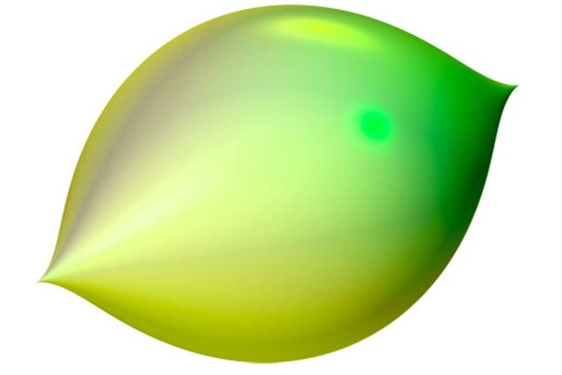
\includegraphics[width=60mm]{limon.jpg}
    \caption{Limón tomado de \url{https://www.elmundo.es/elmundo/2011/01/25/ciencia/1295977576.html} con licencia CC.}
    \label{limon}
\end{figure}

\section{Conclusiones}

En este documento no más se hizo una intro en la sección \ref{intro} y luego ya se me quitaron las ganas de meterle más rollo.

\bibliography{simu}
\bibliographystyle{plainnat}

\end{document}